\documentclass[12pt,a4paper,oneside]{book}
\usepackage[hmargin={1.2in,1.2in},vmargin={1.2in,1.2in}]{geometry}
%%%%%%%%%%%%%%%%%%%%%%%%
\makeindex
\usepackage{textcomp}
\usepackage{fancyhdr}
\usepackage{makeidx}
\pagestyle{myheadings}
\fancyhf{}
\rhead[\leftmark]{thepage}
%%%%%%%%%%%%%%%%%%%%%%%%
\usepackage[utf8]{inputenc}
\usepackage[english]{babel}

%\usepackage{glossaries} % notations & abbreviations
\usepackage{listings} % source code
\usepackage{multicol} % text in 2 columns

\usepackage{array}
\newcolumntype{L}[1]{>{\raggedright\let\newline\\\arraybackslash\hspace{0pt}}m{#1}}
\newcolumntype{C}[1]{>{\centering\let\newline\\\arraybackslash\hspace{0pt}}m{#1}}
\newcolumntype{R}[1]{>{\raggedleft\let\newline\\\arraybackslash\hspace{0pt}}m{#1}}

%images and colors
\usepackage{graphicx}
\usepackage[usenames,dvipsnames]{color}

\usepackage{amsmath, amsthm, amssymb} %definitions
\usepackage{framed} %frames

%ADDITION
\usepackage{graphicx}
\usepackage{tikz}
\usepackage{tkz-graph}
\usetikzlibrary{arrows,shapes}
\usetikzlibrary{external}
\tikzexternalize % activate!

%\usepackage{algorithmicx}
%\usepackage{algpseudocode}
%\usepackage{algorithm}
\usepackage[]{algorithm2e}

\usepackage{float} %option H for placing table,figure,..
\usepackage{svg}
%\usepackage{amsmath}

\usepackage{chngcntr}
\counterwithout{equation}{chapter}

\usepackage{comment}
%\excludecomment{figure}
%\let\endfigure\relax

\definecolor{ref}{HTML}{FF0000}

\newtheorem{mydef}{Definition}
\newtheorem{thm}{Theorem}
\newtheorem{corollary}{Corollary}
\newtheorem{lemma}{Lemma}
\usepackage[final]{pdfpages} % include pdf files


\numberwithin{equation}{chapter}

% Lists of symbols and abbreviations
\usepackage{glossaries}
%\newacronym{st}{s.t.}{such  that}

\newglossaryentry{vertexNumber}{
  name={$n$},
  description={Number of vertices in a graph}
 }
 \newglossaryentry{edgeNumber}{
  name={$m$},
  description={Number of edges in a graph}
 }
 \newglossaryentry{cliqueNumber}{
  name={$\omega(G)$},
  description={The maximum size of a clique of G}
 }
 \newglossaryentry{IndependentNumber}{
  name={$\sigma(G)$},
  description={The maximum size of an independent set of G}
 }
 \newglossaryentry{vertexCoverNumber}{
  name={$\tau(G)$},
  description={The minimum size of a vertex cover of G}
 }
 \newglossaryentry{chromaticNumber}{
  name={$\chi(G)$},
  description={The minimum number of color needed for a valid coloring of G}
 } 
 \newglossaryentry{packingChromaticNumber}{
  name={$\chi_{P}(G)$},
  description={The minimum number of color needed for a valid packing coloring of G}
 }
 \newglossaryentry{BooleanSet}{
  name={$\mathbb{B}$},
  description={The set $\{0,1\}$}
 }
 \newglossaryentry{VerticesSet}{
  name={$V$},
  description={The set of vertices}
 }
 \newglossaryentry{EdgeSet}{
  name={$E$},
  description={The set of edges}
 }
   \newglossaryentry{PathGraph}{
  name={$P_n$},
  description={Path graph on n vertices}
 }
  \newglossaryentry{CycleGraph}{
  name={$C_n$},
  description={Cycle graph on n vertices}
 }
  \newglossaryentry{Hypercube}{
 name={$Q_n$},
 description={Hypercube graph on vectors of size n}
}
\loadglsentries{glossary}
\makeglossaries


\usepackage{hyperref}
\hypersetup{
	bookmarksnumbered = true,
	pdfstartview      = FitH,
	pdfborder         = {0 0 0},
    colorlinks,
    citecolor = blue,
    filecolor=blue,
    linkcolor=blue,
    urlcolor=red,
	pdfauthor   = {Romain Vandemaele},
	pdftitle    = {Packing coloring : study of mixed integer formulations},
	pdfsubject  = {Packing coloring}
	}
\everymath{\displaystyle}

\begin{document}
%%%%%%%%%%%%%%%%
\frontmatter
\begin{titlepage}
\begin{center}
	\textbf{UNIVERSIT\'E LIBRE DE BRUXELLES}\\
	\textbf{Facult\'e des Sciences}\\
	\textbf{D\'epartement d'Informatique}
	\vfill{}\vfill{}

	%\begin{center}
	{\Huge  Packing coloring : study of mixed integers formulations}
	%\end{center}

	{\Huge \par}
	\begin{center}{\LARGE Romain Vandemaele}\end{center}{\Huge \par}
	\vfill{}
	
\includegraphics[keepaspectratio=true,scale=0.2]{figures/ulb.jpg}
	\vfill{}
	\begin{flushright}{\large \textbf{Promoteur :}}\hfill{}{\large Travail pr\'eparatoire au m\'emoire}\\ {\large \href{http://homepages.ulb.ac.be/~bfortz/}{Prof. Bernard Fortz}}\hfill{}
    {pr\'esent\'e en vue de}\\
	{\large l'obtention du grade de}\\
	\hfill{}{\large Master en Sciences Informatiques}\end{flushright}{\large\par}
	\vfill{}\vfill{}\enlargethispage{3cm}
	\textbf{Ann\'ee acad\'emique $2015$~-~$2016$}
\end{center}
\end{titlepage}
\newpage
\thispagestyle{empty}
\null

\newenvironment{vcenterpage}
{\newpage\thispagestyle{empty}
\vspace*{\fill}}
{\vspace*{\fill}\par\pagebreak}
\pagebreak

\begin{comment}
\begin{vcenterpage}
\begin{flushright}
    \large\em\null\vskip1in
        Dedicated to all the future jokes \\
		this part is not obligatory \vfill
  \end{flushright}
\end{vcenterpage}
\end{comment}




\thispagestyle{empty}
\vspace*{5cm}

\begin{quotation}
\noindent ``\emph{Science is what we understand well enough to explain to a computer, Art is all the rest.}''
\begin{flushright}\textbf{Donald E. Knuth\footnote{\url{http://www-cs-faculty.stanford.edu/~uno/}}, 1996}\end{flushright}
\end{quotation}

\medskip

\begin{quotation}
\noindent ``\emph{The purpose of computation is insight, not numbers.}''
\begin{flushright}\textbf{Richard Hamming\footnote{\url{https://en.wikipedia.org/wiki/Richard_Hamming}}, 1962}\end{flushright}
\end{quotation}

%\include{acknowledgments}

\setcounter{page}{0}

\tableofcontents
\listoffigures
\glsaddall
\printglossaries


\mainmatter


%\include{introduction}


\chapter*{Acknowledgements}
\thispagestyle{empty}

I like to acknowledge my advisor Bernard Fortz for its advices.

\clearpage


%----------------------------------------------------------------------------------------

% Define some commands to keep the formatting separated from the content
\newcommand{\keyword}[1]{\textbf{#1}}
\newcommand{\tabhead}[1]{\textbf{#1}}
\newcommand{\code}[1]{\texttt{#1}}
\newcommand{\file}[1]{\texttt{\bfseries#1}}
\newcommand{\option}[1]{\texttt{\itshape#1}}


\tikzstyle{vertex}=[circle,fill=black!35,minimum size=20pt,inner sep=0pt]
\tikzstyle{selected vertex} = [vertex, fill=red!24]
\tikzstyle{edge} = [draw,thick,-]
\tikzstyle{weight} = [font=\small]
\tikzstyle{selected edge} = [draw,line width=5pt,-,green!50]
\tikzstyle{ignored edge} = [draw,line width=5pt,-,red!20]

%----------------------------------------------------------------------------------------

\chapter{Introduction}
\label{sec:introduction}
\section{Notions}

In this document, every graph is an undirected graph and $n$ and $m$ denote respectively the number of vertices($|V|$) and the number of edges($|$\gls{EdgeSet}$|$). Moreover an edge between two vertices $u$ and $v$ is denoted $uv$.


\begin{mydef}
\label{def:distance}
\keyword{The distance between u and v} in a graph G=(V,\gls{EdgeSet}) with $u,v \in V$ noted as $d_{uv}$ is the length of the shortest path from $u$ to $v$. Two vertices are \keyword{adjacent} iff the distance between them is one.
\end{mydef}

\begin{mydef}
\label{def:induceSubgraph}
\keyword{An induced subgraph} of $G = (V,$\gls{EdgeSet}$)$ is a graph $H = (V\prime,E\prime)$ \acrshort{st} $V\prime \subseteq V$ and $uv \in E\prime \iff u,v \in V\prime\ \land\ uv \in $ \gls{EdgeSet}. H is denoted as a subgraph of G induced by $V\prime$. H is induced by $E\prime$ if $E\prime \subseteq E\ \land\ u \in V\prime \iff \exists v \in V\ uv \in E\prime $
\end{mydef}

\begin{mydef}
\label{def:clique}
\keyword{A clique} is a subgraph of G=(V,E) induced by $S \subseteq V $ \acrshort{st} $\forall u,v \in S \text{ with } u \neq v, uv \in E$. The maximum size of a clique in G is denoted here by \gls{cliqueNumber}  and referred as the \textbf{clique} number. If $S=V$ then G is called a clique and denoted $K_n$.
\end{mydef}

\begin{mydef}
\label{def:independent}
\keyword{An independent set} is an subgraph of G=(V,E) induced by $S \subseteq V $  \acrshort{st} $\forall u,v \in S \text{ with } u \neq v, uv \notin E$. The maximum size of a independent set in G is denoted here by \gls{IndependentNumber} and referred as the \textbf{independence number}.
\end{mydef}

\begin{mydef}
\label{def:vertexCover}
\keyword{A vertex cover} of a graph G=(V,E) is a subset $C \subseteq V$ \acrshort{st} $\forall uv \in $\gls{EdgeSet}$, u \in C \lor v \in C$. The maximum size of a vertex cover in G is denoted here by \gls{vertexCoverNumber}.
\end{mydef}

\section{Problem}

The packing coloring is a special case of the famous coloring problem. This problem consists of assigning a color to each vertex of a graph s.t. two adjacent vertices cannot have the same color. Such a coloring is called \textbf{valid}. A  valid coloring of a graph is showed in Figure \ref{fig:graphColored}. Here it is enough to alternate between 2 colors when coloring them in order. This coloring is valid because each vertex is only adjacent to the previous and next vertex modulo 10 and the number of vertices is even so the last vertex colored has not the same color as the first one.

\begin{figure}[h]
\centering
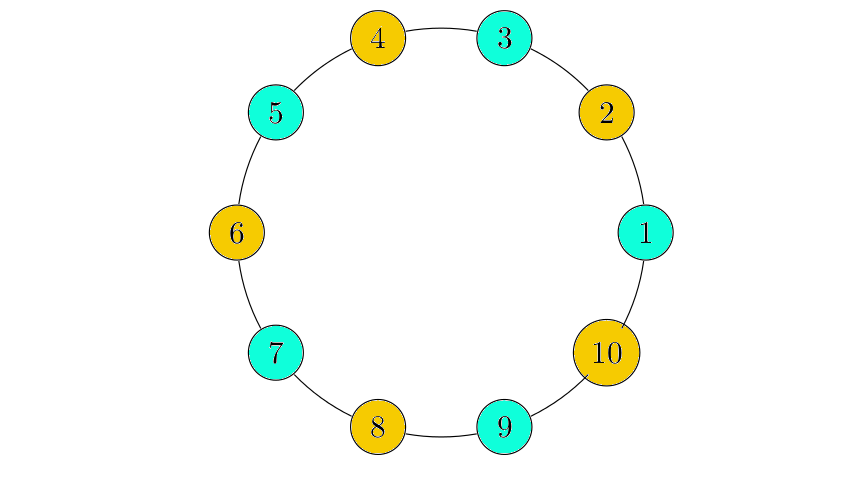
\includegraphics[scale=0.3]{figures/graphColored.png}
\caption{Example of a graph's coloring }
\label{fig:graphColored}
\end{figure}

The packing coloring problem considered here, consists also of a coloring but the constraints are different. Indeed, two vertices having the same color $i$ must have a distance of at least $i+1$. For instance, Figure \ref{fig:graphPackingColored} presents a valid packing coloring of a graph with this correspondence between colors and their number in Table \ref{tab:colors}  :



In this case, more colors are needed than with the coloring by using twice the minimal number of colors to obtain a valid coloring. On both figures, only one valid coloring is shown but there can have a large amount of them even with the minimal number of colors. For instance, the colors can be rotated s.t. vertex $i$ has the color of vertex $i + j mod n$ with $j \in \mathbb{Z}$.

\begin{figure}[H]
\centering
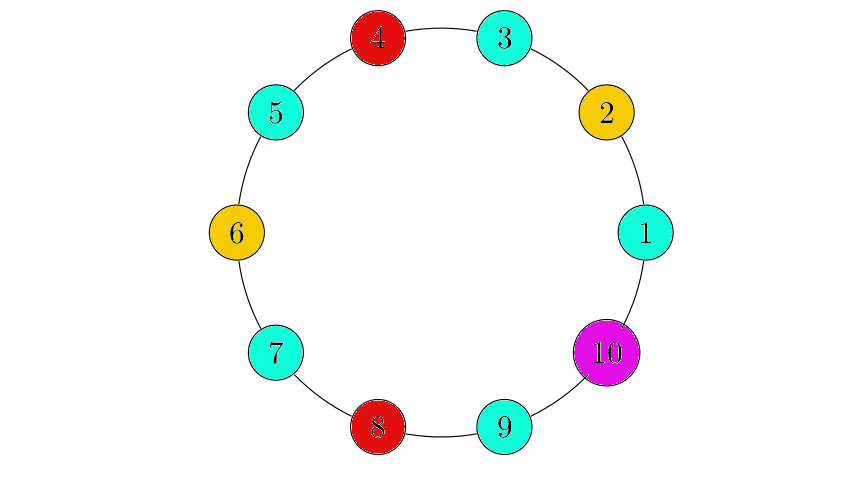
\includegraphics[scale=0.3]{figures/graphPackingColoredV2.png}
\caption{Example of a graph's packing coloring}
\label{fig:graphPackingColored}
\end{figure}

\begin{table}[H]
\centering
\begin{tabular}{|c|c|c|c|c|}
\hline
Number & 1 & 2 & 3 & 4\\
\hline
Color\footnote{obtained from \url{http://gauth.fr/2011/09/get-a-color-name-from-any-rgb-combination/}} &  Bright turquoise & Yellow (Munsell) & KU Crimson & Phlox\\
\hline
\end{tabular}
\caption{The correspondence of colors in Figure\ref{fig:graphPackingColored}.}
\label{tab:colors}
\end{table}

\section{Description}

Now that the subject is introduced, the next sections enter in greater details about colorings. The most important results and formulations of the coloring problem are presented in Section \ref{sec:coloring}. The Section \ref{sec:packing coloring} follows the same structure by extending results of section \ref{sec:coloring} if possible but specific results about this problem are also presented.


\chapter{Coloring}
\label{sec:coloring}

\section{Description}
\label{sec:coloring_description}

The problem was briefly described in Section \ref{sec:introduction}, the goal is to find a function $f$ that assigns colors to every vertex of a graph $G=(V,$\gls{EdgeSet}$)$ defined as follow :

\begin{equation}
\begin{aligned}
f : V \longrightarrow C \\
f(u) \neq f(v)\ \forall\ uv \in E \\
C \subseteq \mathbb{N} \\
\end{aligned}
\end{equation}

There is two main ways to see the problem. On one hand, a decision problem which is a problem where the response is either yes either no. The question is whether $G$ has a valid coloring with $k$ color or not. For this question $k$ is either an input as $G$ or is fixed which influences its complexity. If $k$ is fixed then it is enough to test all $nk$ possible coloring which is polynomial in the input size. This problem defines a set of languages $L = \{L_i\ \forall i \in \mathbb{R} \}\ $ with  $L_k = \{ <G> : \text{G has a valid coloring with k colors} \}\ $ with $<G>$ a binary encoding of $G$.\\
On the other hand, an optimization problem where the goal is to minimize or maximize an objective function $g$ under some constraints on variables. For example, $|C|$ has to be minimized also called the chromatic number under the constraint that the coloring is valid. Some concrete examples are described in Section \ref{sec:coloring_formulations}.\\

\begin{mydef}
\label{def:ChromaticNumber}
\keyword{The chromatic number} of a graph G, denoted \gls{chromaticNumber}, is the minimum number of colors needed for a valid coloring of a graph G.
\end{mydef}

\begin{mydef}
\label{def:planarGraph}
\keyword{A planar graph} is a graph that can be drawn s.t. there is no crossings between the edges and between a vertex and an edge. The graph has to be drawn s.t. each vertex is represented as a unique point in $\mathbb{R}^2$ and edges are represented as lines between the 2 corresponding points.
\end{mydef}

This problem has many applications like the coloration of a map s.t. two neighboring countries have different colors to be able to distinguish the frontiers. In 1977, Kenneth Appel and Wolfgang Haken\footnote{A shorter proof was made in \cite{4color}} proved first the four color Theorem in \cite{appel1977} that states that for any planar graph G \gls{chromaticNumber} $\leq 4$.



\section{Results}
\label{sec:coloring_results}

There are several results on this very popular problem, the most general ones are presented here.

\subsection{Complexity}

\begin{thm}
\label{thm:NP-complete1}
The coloring problem is NP-complete
\end{thm}

\begin{proof}
The decision problem belongs to the NP class. Indeed, a poly-time verifier would take the neighborhood of every vertex and test if the constraint is respected. This verifier would be in $\mathcal{O}(n+m)$. For the NP-hard property, a proof by reduction from $3-SAT$ is in \cite{Complexity}\footnote{In the version with exercise correction}.
\end{proof}

Theorem \ref{thm:NP-complete1} implies that no polynomial algorithm exists until proven otherwise\footnote{P = NP ?}.

\subsection{Lower and Upper bounds}
\begin{thm}
\label{thm:LB-UB}
For any graph $G=(V,$\gls{EdgeSet}$)$,  \gls{cliqueNumber}$ \leq $ \gls{chromaticNumber} $\leq n$.
\end{thm}

\begin{proof}
For the upper bound, it is easy to observe that there cannot be more than $n$ colors because each vertex is associated with one and only one color. \\
The lower bound is proved by contradiction. Suppose  \gls{chromaticNumber} $ < $ \gls{cliqueNumber} then two vertices $u$ and $v$ in a clique of size \gls{cliqueNumber} have the same color by the pigeonhole principle but by the definition of a clique $u$ and $v$ are adjacent.
\end{proof}

This is very general bounds it can be reduced by taking independent set into account because every vertex in an independent set can be colored by the same color without breaking any constraints. Thereby the upper bound can be reduced as stated in Theorem \ref{thm:LB-UBStable}.

\begin{thm}
\label{thm:LB-UBStable}
For any graph $G=(V,E)$, \gls{chromaticNumber} $ \leq |S| + n - \displaystyle\sum_{s \in S} |s| $.
\[S = \{s_1,s_2,\dots,s_n | s_i\text{ is an independent set }\forall i \in \{1,\dots,n\} \land  s_i \cap s_j = \emptyset\ \forall i,j \in \{1,\dots,n\}\ i \neq j \} \]

We take $S$ having the maximal $\displaystyle\sum_{s \in S} |s|$ among all set having this property.

\end{thm}

\begin{proof}
All set of $S$ are independent so each one can be colored with a unique color thus it uses $|S|$ color at most. We still have to color $n - \displaystyle\sum_{s \in S} |s| $ vertices. In the worst case, each of them will have one unique color. \\
\end{proof}

The upper bound can still be reduced by using the vertex cover number ,\gls{vertexCoverNumber} by observing its links with independent set :

\begin{thm}(Gallai's)
\label{thm:Gallai}
For any graph $G = (V,$\gls{EdgeSet}$)$, $n - \sigma(G) = $ \gls{vertexCoverNumber}.
\end{thm}

\begin{proof}
Let $C$ be a minimum vertex cover, the set $I = V \setminus C$ is an independent set. If $|I| \leq 1$ then it is trivial. Otherwise, by contradiction suppose that there exists $a,b \in I$ that are adjacent and let $e$ the edge between $a$ and $b$. Then $e$ is not covered by $C$ which contradicts our hypothesis that $V$ is a vertex cover. By the same idea, the complement of an independent set is a vertex cover.\\
We still have to prove that $I$ is a maximum independent set. By contradiction, let $I\prime$ be an independent set s.t. $|I| < |I\prime|$ then $C\prime = V \setminus I\prime$ is a vertex cover with $|C\prime| < |C|$ but $C$ is a minimal vertex cover.
\end{proof}

By Theorem \ref{thm:Gallai} and Theorem \ref{thm:LB-UBStable}, corollary \ref{crl:VC} can be proved easily.

\begin{corollary}
\label{crl:VC}
For any graph $G=(V,E)$, \gls{chromaticNumber} $ \leq $ \gls{vertexCoverNumber}$ + 1$.
\end{corollary}


\section{Formulations}
\label{sec:coloring_formulations}

This sections presents several formulation of the optimization problem. There exists several formulations with distinct number of variables and constraints.

\section{Vertex color}
\label{VC}
This first formulation is the more intuitive one, there is a boolean variable $x_{ic}$ for every vertex $i$ and color $c$ thereby the number of variables  is in $ \mathcal{O}(n^2)$ because there are at most $n$ colors as proved in Theorem \ref{thm:LB-UB}.

\[\forall i \in V \forall c \in C\  x_{ic} =
  \begin{cases}
    1       & \quad \text{if the color of vertex i is c}  \\
    0  & \quad \text{otherwise }\\
  \end{cases}
\]

In addition to the constraint on adjacent vertices, the fact that a vertex must have exactly one color must be ensured. This gives the following formulation :

\begin{eqnarray}
  minimize\ & z & \label{VC:FE} \\
  subject\ to & \displaystyle\sum_{c=0}^{n}{x_{ic}} = 1 & \forall i \in V \label{VC:C1} \\
  &  x_{ic} + x_{jc} \leq 1 & \forall ij \in E,\ \forall c  \in C \label{VC:C2}\\
  &  x_{ic} c \leq z & \forall c  \in C,\ \forall i \in V \label{VC:C3}\\
  &  x_{ic} \in \mathbb{B} &  \forall i \in V,\ \forall c  \in C \label{VC:C4}\\
  &  z \in \mathbb{Z} &
\end{eqnarray}

In the objective function \ref{VC:FE}, $z$ represent the number of color used which is the number to minimize. Constraint \ref{VC:C1} implies that each vertex has one and exactly one color. Constraint \ref{VC:C2} implies the condition on adjacent vertices because if they have the same color the sum would be 2. Finally, constraint \ref{VC:C3} implies that if color $c \in \mathbb{N}$ is used then $z$ is at least $c$. In other words, $z$ cannot be lower than the larger color used and cannot be greater because it is minimized so $z$ is well-defined.

\begin{mydef}
\keyword{The density} of a graph G=(V,\gls{EdgeSet}) is the number of edges compared to the maximum number of edges possible.
\[density = \frac{2|E|}{|V|(|V|-1)}\]
\end{mydef}


\[ \text{The  number of constraints is  } \mathcal{O}(n + nm + n^2  ) =
  \begin{cases}
    \mathcal{O}(nm)       & \quad \text{if density } > \frac{2}{n}  \\
    \mathcal{O}(n^2)      & \quad \text{otherwise }\\
  \end{cases}
\]



A problem is that this formulation is \keyword{symmetric} which means that several solutions are equivalent. Suppose we have a graph which is a clique of size 5. The two results $z=5,\ x_{11}=1,\ x_{22}=1,\ x_{33}=1,\ x_{44}=1,\ x_{55}=1$ and  $z=5,\ x_{11}=1,\ x_{22}=1,\ x_{33}=1,\ x_{45}=1,\ x_{54}=1$ ,represented only by the variables which are true, are equivalent. Indeed, each vertex has exactly one unique color in both solution. This may cause problems when resolving it by branch and bound which is a technique to reduce the set of solutions to explore by applying bounds. This technique implies imposing values to variables to reduce possibilities for the others but forcing a color on a vertex here could lead to an equivalent solution.


\section{Independent set}
\label{IC}

\begin{mydef}
A \textbf{partition} of a set $A$ is a set $P=\{A_1,A_2,\dots,A_n | A_i \subseteq A\ \forall i \in \{1,2,\dots,n\} \}$ of subsets s.t. $A_i \cap A_j = \emptyset\ \forall i,j \in\{1,2,\dots,n\}\ i \neq j $ and $\bigcup_{i \in \{1,2,\dots,n\}} A_i = A$.
\end{mydef}

Firstly, we can observe that a coloring creates a partition of $V$ with $P_1,P_2,\dots,P_{\chi}$ as subsets s.t. each vertex has the same color as every vertices that are in the same subset and has a different color than every vertex that is in a different subset. Moreover, a vertex has one color so is in exactly one subset. Each subset is an independent set because there cannot be any edges between two vertices having the same color. \\

From this observation, a formulation can express the fact that an independent set is taken as a partition. Let $I$ be the set of independent set, the variable x is defined as follows :

\[ \forall i \in I\ x_{i} =
  \begin{cases}
    1       & \quad \text{if the independent set i is taken as a partition}  \\
    0  		& \quad \text{otherwise }\\
  \end{cases}
\]

\begin{eqnarray}
minimize\ &  \displaystyle\sum_{i \in I} x_i & \label{IC:FE}\\
subject\ to &   \displaystyle\sum_{i \in I | v \in i}{x_{i}} = 1   & \forall v \in V  \label{IC:C1}\\
&  x_{i} \in \mathbb{B} &  \forall i \in I
\end{eqnarray}

In the objective function \ref{IC:FE} the number of partitions is minimized which is equal to the number of colors. The constraint \ref{IC:C1} states that the sum of $x_i$ for every independent set $i$ containing a vertex $v$ is one thereby a vertex is in one and only one chosen independent set. Compared to \ref{VC}, there are less constraints more precisely $n$ but far more variables. Indeed, there is $\mathcal{O}(2^n)$ variables because in the worst case, every subset is an independent set. \\

This number can be reduced by taking into account only the independent set which are maximal which implies that no vertex can be added to them without keeping them an independent set. Suppose that in the solution there is an independent set $S$ which is not maximal. Thereby, there exists a vertex $v$ that can be added to $S$ and keep it independent. The new set is denoted $S\prime = S \cup \{v\}$. The solution can be modified to take $S\prime$ instead of $S$ and replace $T$ the independent set taken that contains $v$ by $T\prime= T - v$. We can do that because $S\prime$ and $T\prime$ were not taken in the original solution because it will not respect constraint \ref{IC:C1}. \\

Its exponential number of variables is an important drawback but some technique like column generation can facilitate the computations. Indeed, a column generation or branch and price algorithm for the multi-coloring problem is described in \cite{BranchAndPrice}. In this another variant, each vertex is associated to a set of colors. Two sets of two adjacent vertices must have an empty intersection. The case when the set has a cardinality of one is the classical coloring thus multi-coloring is a generalization of the famous problem. Another inconvenient of this formulation is that finding an independent set is also NP-complete(cf. \cite{Complexity} for a proof).

\section{Representative vertex}
\label{sec:RV}

There exists another formulation with less variables than \ref{IC} and conserving the same amount of constraints of \ref{VC}. As its name implies, there are representative which are vertices that represent a color. There is only one representative per color.
From this idea, the variables $x$ is derived :

\[\forall u,v \in V\ x_{uv} =
  \begin{cases}
    1       & \quad \text{if $u$ represents the color of $v$}  \\
    0  		& \quad \text{otherwise }\\
  \end{cases}
\]

A coloration is derived in 2 steps. First, find all representatives $u_1,u_2,\dots, u_{\chi} \in V$ s.t. $x_{uu}=1$ and assign them a different color. Finally, the color of $v \in V$ is the color of its representative vertex $u_i \in V$ s.t. $x_{u_{i}v}=1$. The formulation is as follow

\begin{eqnarray}
minimize\ & \displaystyle\sum_{u \in V}  x_{uu}& \label{RV:FE} \\
subject\ to & \displaystyle\sum_{u \in V} x_{uv} = 1 & \forall v \in V\ \label{RV:C1}\\
& x_{uv} + x_{uv\prime} \leq x_{uu} & \forall u \in V\ \forall vv\prime \in E \label{RV:C2}\\
&  x_{uv} \in \mathbb{B} &  \forall u,v \in V
\end{eqnarray}

The objective function \ref{RV:FE} minimizes the number representatives thus also the number of colors. Constraint \ref{RV:C1} states that each vertex has one and only one representative and constraint \ref{RV:C2} implies that two adjacent vertices cannot have the same representative and that if a vertex $u$ represents another one, $x_{uu}$ is forced to one. There is $n^2$ variables and $n + nm = \mathcal{O}(nm)$ constraints. We have the same performance as \ref{VC} but the number of constraints can still be reduced in some cases.

\begin{mydef}
\label{def:neighbourhoodVertex}
\keyword{The neighborhood $N$ of a vertex $u$} in a graph $G=(V,E)$ is the set of vertices that are adjacent to $u$.
\[N(v) = \{v\in V \setminus \{u\} | uv \in E \}\]
\end{mydef}


\begin{mydef}
\label{def:neighbourhoodSubset}
\keyword{The neighborhood $N$ of $S \subseteq V$} in a graph $G=(V,E)$ is the set of vertices that are adjacent to a vertex in $S$ but are not in $S$.
\[N(S) = \{v\in V \setminus S | \exists u \in S\ uv \in E\  \}\]
\end{mydef}

\begin{mydef}
\label{def:antiNeighbourhoodSubset}
The \textbf{ anti-neighborhood} $\bar{N}(S)\ for\ S \subseteq V$ is the set of vertices not accessible from a vertex in $S$ via only one edge.
\[\bar{N}(S) = \{ v \in V \setminus S | uv \notin E ,\forall u \in S \}\]
\end{mydef}

The anti-neighborhood can also be defined as the neighborhood in the complementary graph. The anti-neighborhood is very useful for coloring because $\bar{N}(u)$ defines the set of vertices that can be represented by $u$ which reduces the number of constraints. Thereby, we can restricted our variables $x_{uv}$ to all pair $u \in V\ and\ v \in \bar{N}(u) \cup u$ which gives us $\mathcal{O}(n^2)$ but in practice it is going to be less than $n^2$ because it's only the case when each vertex has an empty neighborhood. This gives us the following formulation from \cite{polytope} :

\begin{eqnarray}
minimize\ & \displaystyle\sum_{u \in V}  x_{uu}& \\
subject\ to & \displaystyle\sum_{u \in \bar{N}(V)} x_{uv} = 1 & \forall v \in V \\
& x_{uv} + x_{uv\prime} \leq x_{uu} & \forall u \in V\ \forall vv\prime \in E(\bar{N}(u)) \\
&  x_{uv} \in \mathbb{B} &  \forall u \in V,\ v \in \bar{N}(u)\cup u
\end{eqnarray}

That gives us $\mathcal{O}(n + n\bar{m})$ with $\bar{m}$ the number of edges in the complementary graph which is better if the original graph has a high density. This formulation like the one in Section \ref{VC} is symmetric because the solution is the same if only the representatives of some partitions change. For instance, if $u \in V$ represents $v_1,v_2,v_3,\dots,v_n$ then $\{v_1,v_2,v_3,\dots,v_n,u\}$ forms an independent set and is also a partition, $v_i$ could become the representative for $v_1,v_2,v_3,\dots,v_{i-1},v_{i+1},\dots,v_n,u$ and have exactly the same coloring. One solution proposed by \cite{AsymetricRepresentation} is to impose a total order on the vertices and define a deterministic rule to determine the representative of an independent set. \\

This formulation is often used as base for algorithms on formulations. For example \cite{BranchAndCut} presents a branch and cut algorithms to solve a special case of the coloring problem named equitable  coloring. In This variant, the difference in cardinality of two partitions as defined in section \ref{IC} must be at most one. Figure \ref{fig:graphColored} represents an equitable coloring because there is exactly 5 vertices for each color. If a third color was used to recolor only one vertex then the coloring would not be equitable anymore. Indeed, a color would have one vertex and another one would have 4 vertices which makes a difference of 3. \\

%----------------------------------------------------------------------------------------

\chapter{Packing coloring}
\label{sec:packing coloring}

\section{Description}

The problem was first introduced by \cite{broadcastchromatic} as \textit{broadcast coloring}. The problem was about assigning a frequency to radio antennae. The problem comes from the interference that occurs when two signals with same frequency are too close. There are several signal's power that indicates the minimal distance between two signals with same frequency. There is a correspondence between a frequency and a color. Moreover, the number associated to the color increase with the power of the frequency. Then, several other applications were found  like animals' placement. Thereby, this notion was renamed to the one of \textit{packing coloring} by \cite{PCNLatice}. This come from the notion of \keyword{i-packing} which is a set of vertices having the property that the distance between each pair of distinct vertices have a distance of at least $i + 1$. For example an independent set is a $1-packing$. As said in Section \ref{sec:introduction}, this problem is also about finding a coloring described by a function $f$ :

\begin{equation}
\begin{aligned}
f : V \longrightarrow C & \\
\forall\ uv \in E\ f(u) = f(v)\  \implies  d_{uv} > f(u) &\\
C \subseteq \mathbb{N} & \\
\end{aligned}
\end{equation}

The decision and optimization problems are equivalent to the coloring problem by deciding if a valid packing coloring with $k$ colors exists and minimizing the number of color used. In the same way, the notion of chromatic number is extended to the packing chromatic number denoted \gls{packingChromaticNumber}. \\

\section{Results}
\label{sec:PCresults}
This decision problem has been proved to be NP-complete by \cite{broadcastchromatic} except if $k \leq 3$. We denote a valid packing coloring with $k$ colors by a \keyword{k-coloring}. Nonetheless, there are several kind of graphs where the packing chromatic number can be bounded. This section is dedicated to present this type of results found in the literature.


\subsection{General bounds}

The bounds presented in Theorem \ref{thm:LB-UB} are still correct. Nonetheless \gls{chromaticNumber} and \gls{packingChromaticNumber} are not independent by Theorem \ref{thm:gBound}.


\begin{thm}
\label{thm:gBound}
For any graph G, \gls{chromaticNumber} $\leq $ \gls{packingChromaticNumber}.
\end{thm}

\begin{proof}
Every valid packing coloring is a valid coloring thus if a packing coloring with fewer colors than \gls{chromaticNumber} is found then a better coloring has been fond thus contradicting the definition of $\chi_(G)$.
\end{proof}

\begin{mydef}
\label{def:splitGraph}
\keyword{A split graph} $G=(V,E)$ is a graph in which $V$ can be partitioned in $A$ and $B$ s.t. $A$ induces a clique and $B$ induces an independent set.
\end{mydef}

This is not a strict lower bound so there also exists graphs with $\chi = \chi_P$ like split graphs. In both coloring, each vertex of the partition $A$ has to take an unique color and the ones from $B$ can have the same color which is not used in $A$ except if there is no edge between $A$ and $B$ in which case a color from $A$ van be reused for vertices in $B$.



\subsection{Graphs with low packing chromatic number}

This section considers graphs that need only a few colors to have a valid packing coloring like path graphs, cycle graphs and star graphs.

\begin{mydef}
\keyword{A path graph} denoted \gls{PathGraph} is composed of $n$ vertices $v_1,v_2,\dots,v_n$ s.t. $v_iv_j \in E \Rightarrow j = i+1$ except if $i=n$.
\end{mydef}

\begin{mydef}
\label{def:cycleGraph}
\keyword{A cycle graph} \gls{CycleGraph} is composed of only a cycle on $n$ vertices $v_1,v_2,\dots,v_n$ s.t. $v_iv_j \in E \Rightarrow j = i+1 mod n$.
\end{mydef}

A path graph is very simple and can be colored with only a few of colors as stated by Theorem \ref{thm:Path}. Theorem \ref{thm:cycleGraph} states an equivalent proposition for \hyperref[def:cycleGraph]{cycle graphs}.

\begin{thm}(by \cite{broadcastchromatic})
\label{thm:Path}
For any path graph \gls{PathGraph}, $\chi_P($\gls{PathGraph}$) \leq 3$.
\end{thm}

\begin{proof}
If $n \geq 4$, \cite{broadcastchromatic} found a pattern that results in a valid packing coloring which is
\[1 2 1 3 1 2 1 3 1 \dots \] as illustrated in Figure \ref{fig:path}
This pattern uses only 3 colors. This pattern is optimal because at most $\frac{n}{2}$ vertices can be colored by 1 and at most $\frac{n}{3}$ vertices by 2 with coloring $\frac{n}{3} + \frac{n}{2}$ vertices is impossible because of overlapping. If $n < 4$, the pattern can still be used which results in a 1-coloring or 2-coloring depending on $n$.
\end{proof}

\begin{figure}[h]
\centering
\begin{tikzpicture}

   \foreach \pos/\name/\label in {{(-2,0)/a/1}, {(0,0)/b/2}, {(2,0)/c/1},
                             {(4,0)/d/3}, {(6,0)/e/1}, {(8,0)/f/2},{(10,0)/g/1},{(12,0)/h/3}}
         \node[vertex] (\name) at \pos {$\label$};

  \foreach \source/ \dest  in {a/b, b/c,c/d,d/e,e/f,f/g,g/h}
        \path[edge] (\source) -- node[weight] {} (\dest);
 \end{tikzpicture}
\caption{Optimal packing coloring of a path graph}
\label{fig:path}
\end{figure}



A coloring and a packing coloring of a cycle graph are illustrated respectively on Figure \ref{fig:graphColored} and \ref{fig:graphPackingColored}.

\begin{thm}(by \cite{broadcastchromatic})
\label{thm:cycleGraph}
For any cycle graph \gls{CycleGraph}, if $n  \geq 3$ and $n$ is 3 or a multiple of 4, then $\chi_P($\gls{CycleGraph}$) = 3$; otherwise $\chi_P($\gls{CycleGraph}$) = 4$.
\end{thm}

\begin{proof}
(Proof idea)
A cycle graph \gls{CycleGraph} can be seen as \gls{PathGraph} in which its two endpoints are linked together with an edge. We could use the pattern described above and then link the endpoints but it can break the coloring. The case $n \leq 3$ being trivial, we consider $n$ as a multiple of 4 then the last vertex completes a pattern thus by linking it to the beginning we create a chain of complete patterns so the coloring is valid as proved by Theorem \ref{thm:Path}. \\
In the other cases, some changes  have to be done which implies adding a fourth color. In all cases enumerated below, the last vertex is now colored by 4 as illustrated in Figure \ref{fig:graphPackingColored} :

\begin{itemize}
\item $n = 4r + 1$ : \textcolor{red}{1}  2 1 3 \dots 1 2 1 3 \textcolor{red}{1}  $\longrightarrow$  1 2 1 3 \dots 1 2 1 3 \textbf{4}
\item $n = 4r + 2$ : 1 2 1 3 \dots 1  \textcolor{red}{2}  1 3 1 \textcolor{red}{2} $\longrightarrow$  1 2 1 3 \dots 1 2 1 3 1 \textbf{4}
\item $n = 4r + 2$ : \textcolor{red}{1} 2 1 3 \dots 1 2 1 3 1 2 \textcolor{red}{1} $\longrightarrow$  1 2 1 3 \dots 1 2 1 3 1 2 \textbf{4}
\end{itemize}

\end{proof}

\begin{mydef}
\label{def:starGraph}
\keyword{A star graph} is a graph denoted $S_n$ that have one central vertex which have $n-1$ adjacent vertices that have the central vertex as only neighbor. It also is a tree with $n-1$ leave and with maximum diameter 2.
\end{mydef}

At the beginning of Section \ref{sec:PCresults}, it is mentioned that the decision problem is not NP-hard when $k \leq 3$. This results for $k=2$ comes from star graphs that are the only graphs with $\chi_P = 2$.


\begin{thm}(By \cite{broadcastchromatic})
For any graph G, \gls{packingChromaticNumber} $ = 2 \iff $ G is a star graph.
\end{thm}

\begin{proof}
$(\Leftarrow)$ A coloring is simply applying the color 2 to the central vertex and $1$ to every leaves.\\
$(\Rightarrow)$ $\chi_P(G)=2$ thus $P_4$ is not a subgraph of $G$ because it needs 3 colors by Theorem \ref{thm:Path} thereby  $diam(G) \leq 2$. Moreover, the vertex cover number is $1$ by corollary \ref{crl:VC}. It results that the only graphs that have all these properties are star graphs.\\
\end{proof}

\begin{mydef}
\label{def:bipartite}
A graph G=(V,E) is \keyword{bipartite} if V can be be partitioned in 2 partitions $A$ and $B$ s.t. every edge has one endpoint in $A$ and the other in $B$.
\end{mydef}

\begin{mydef}
\label{def:multigraph}
A \keyword{multigraph} is a graph in which there can be several edges sharing the same endpoints.
\end{mydef}

The last case to consider is when $k=3$, every graph $G$ with \gls{packingChromaticNumber} $=3$ can be created with the following procedure :

\begin{enumerate}
\item Start with a bipartite multigraph with bipartition $A$ and $B$.
\item Subdivide once each edge by adding a vertex between its two endpoints.
\item Add leaves in the original set of vertices $A \cup B$.
\item Do a T-add on vertices in $B$. A T-add is defined in \cite{broadcastchromatic}. This is the operation performed on a vertex $v$ which add a vertex $w$ and an independent set $X$ to the graph. Then an edge between $v$ and $w$ is added as well as a subset of all the possible edges between $X$ and $\{v,w\}$. One example is illustrated in Figure \ref{fig:Tadd} with $X=\{a,b,c,d\}$. On this figure, green edges are added and red ones are not.
\end{enumerate}



\begin{figure}
\centering
\begin{tikzpicture}
\foreach \pos/\name/\label in {{(2,2)/v/3}, {(2,4)/w/1}, {(6,0)/a/1},
                             {(6,2)/b/1}, {(6,4)/c/2},{(6,6)/d/1}}
         \node[vertex] (\name) at \pos {$\name$};

  \foreach \source/ \dest  in {v/w}
        \path[edge] (\source) -- node[weight] {} (\dest);

 \foreach \source/ \dest  in {v/a,v/d,v/b,w/c}
        \path[selected edge] (\source) -- node[weight] {} (\dest);

 \foreach \source/ \dest  in {v/c,w/a,w/b,w/d}
        \path[ignored edge] (\source) -- node[weight] {} (\dest);

 \end{tikzpicture}
\caption{Example of a T-add}
\label{fig:Tadd}
\end{figure}

\subsection{Distance graph}

\begin{mydef}
\label{def:distanceGraph}
A \keyword{distance graph} is a graph $G =(V,E)$ and a distance set $D$ with $V \subseteq \mathbb{Z}$ and $D \subseteq \mathbb{Z^{+}}$ in which each element of $V$ represents a vertex and $E=\{ij | i,j \in V \land |i-j| \in D \}$.
\end{mydef}

In this section, we consider \textbf{infinite distance graphs} which have $\mathbb{Z}$ as vertex set denoted by $D(d_1,d_2,\dots,d_k)$ with the distance set $D = \{d_1,d_2,\dots,d_k\}$. The results from the study of the packing coloring number of these graph in \cite{DistanceGraph} are presented in this section. They found several bounds for when $|D|=2$ as presented :

\begin{enumerate}
\item If $k,t$ are coprime (Recall that 2 integers are coprime iff one is their only common divisor) :
\begin{enumerate}
\item $t$ and $k$ are both odd and $t \geq 825$ then $\chi_P(D(k,t)) \leq 30$.
\item $k$ is odd and $t \geq 898$ is even then $\chi_P(D(k,t)) \leq 56$.
\item $k$ is even and $t \geq 923$ is odd then $\chi_P(D(k,t)) \leq 56$.
\end{enumerate}
\item If $D(k,t)$ is connected and $t \geq 9$ then $\chi_P(D(k,t)) \geq 12$.
\end{enumerate}

In addition, they found bounds for graph with small $k$ and $t$ by finding repeatable patterns(upper bounds) or simply by brute-force(lower bounds) with programs they developed. These results are available on the page \url{http://le2i.cnrs.fr/o.togni/packdist/}. This method is very inefficient because if can take a lot of time. For instance it took them 179 hours to find the lower bounds when $k=3$ and $t=7$. A more efficient technique is to use a formulation like they did in \cite{PCModel} with the one presented in Section \ref{sec:PF_Form}. They found new bounds and improved some of those found previously.

\subsection{Trees}
\label{sec:PC_trees}
Concerning trees, \cite{broadcastchromatic} left as open question to determine if there is a polynomial algorithm to compute $\chi_P$ for any tree. \cite{PCNLatice} suggest that the response was negative by trying two natural approaches but failed. Finally \cite{PCComplexity} has proved that it is NP-complete even for trees although a classic coloring of a tree is trivial. \\

Nonetheless, \cite{Sloper} proved that $\chi_P$ of trees with maximum degrees 3 is bounded by 7 but also that there is no upper bound once that that maximum degree is above 3. there is a similar situation with diameters as proved by \cite{broadcastchromatic}. \\

Indeed, a tree with diameter 3 has a valid packing coloring with 3 colors like illustrated in Figure \ref{fig:treeD3}. The root can be colored $3$, its children $1$. Among its child only one vertex $v$ can have children otherwise the distance between two of these children would be 4. The children of $v$ must have color $1$ because the distance between them is $2$. It creates a problem with $v$ which has also color $1$ but $v$ can be recolored with $2$. Likewise, there is no bounds for trees with diameter 4 but the packing chromatic number can be computed in polynomial time by result from Theorem \ref{thm:Tree4}. \\



\begin{figure}
\centering
\begin{tikzpicture}
\foreach \pos/\name/\label in {{(4,2)/a/3}, {(2,2)/b/1}, {(6,2)/c/1},
                             {(4,0)/d/1}, {(4,4)/e/2}, {(2,4)/f/1},{(6,4)/g/1},{(4,6)/h/1}}
         \node[vertex] (\name) at \pos {$\label$};

  \foreach \source/ \dest  in {a/b, a/c,a/d,a/e,e/f,e/g,e/h}
        \path[edge] (\source) -- node[weight] {} (\dest);
 \end{tikzpicture}
\caption{Optimal packing coloring of a tree with diameter 3}
\label{fig:treeD3}
\end{figure}


\begin{thm}
\label{thm:Tree4}
Let T be a tree with diameter 4 and a central vertex $v$. Let $n_i \forall i \in \{1,2,3\}$ denotes the number of neighbors of degree $i$ of $v$. A vertex is \keyword{large} if its degree is at least 4. Let $L$ be the number of large vertices in the neighborhood of $v$ then :

\[ \text{If } L=0, \chi_P(T) =
  \begin{cases}
    4  & \quad \text{if $n_3 \geq 2$ and $n_1 + n_3 \geq 3$}  \\
    3  & \quad \text{otherwise }\\
  \end{cases}
\]


\[ \chi_P(T) =
  \begin{cases}
    L + 3      & \quad \text{if $n_3 \geq 1$ and $n_1 + n_2 + n_3 \geq 2$}  \\
    L + 1  & \quad \text{if $n_1 + n_2 + n_3 = 0$ }\\
    L+2 & \quad \text{otherwise}
  \end{cases}
\]
\end{thm}


However, \cite{PCComplexity} found a polynomial algorithm for trees with $n$ vertices in $\mathcal{O}(n^{2t+3})$ with $t$ a parameter of the S-packing coloring which is a generalization of the packing coloring. In this one the number of each color is determined by a non decreasing sequence $S= (s_1,s_2,\dots)$ where color $i$ is associated with $s_i$. The packing coloring is the instance where $S=(1,2,3,\dots)$. The algorithm is for the decision problem when $S$ is bounded by a constant $t$ which is not the case for the packing coloring. Nevertheless, the packing chromatic number can be bounded for tress as stated by Theorem \ref{thm:treeBound} from \cite{broadcastchromatic}. \\

\begin{thm}
\label{thm:treeBound}
For any tree T with $n$ vertices, $\chi_P(T) \leq \frac{n+7}{4}$ ,except when $n=4$ or $n=8$ in which case the bound is $\frac{n}{4} + 2$.
\end{thm}

\subsection{Treewidth}

\begin{mydef}
\keyword{A tree decomposition} of a graph $G=(V,E)$ is a tree $T$ and a set $\{T_v\} \subseteq T $ of subtrees for each $v \in V$ such that $\forall v_1,v_2 \in V\  v_1v_2 \in E \Longrightarrow T_{v_{1}} \cap T_{v_{2}} \neq \emptyset $.\newline
\end{mydef}

\begin{mydef}
The \keyword{width} of a tree decomposition $T$ of $G$ is the maximum over all nodes $x \in V(T)$ of the number of subtrees in which $x$ is in minus 1. More formally,
\[ \max_{x \in V(T)} \mid \lbrace v \in V(G)  : x \in V(T_v) \rbrace \mid - 1 \]
\end{mydef}

\begin{mydef}
The \keyword{treewidth} of a graph G, denoted $tw(G)$, is the minimum width over all tree decomposition of G.
\end{mydef}

This notion can be seen as an evaluation of how close a graph is from a tree. Several NP-hard problems like finding a maximum independent set , can be solved in polynomial time for type of graphs with bounded treewidth. For example, trees are the only graphs with treewidth $1$. The (S-)packing coloring problem is one of these NP-hard problems. Some special cases listed below can be solved with a polynomial time algorithm.

\begin{enumerate}
\item The packing coloring when $k$ is fixed proved by \cite{PCComplexity}.
\item The packing coloring when the diameter is also bounded proved by \cite{PCComplexity}.
\item The S-packing coloring when S is bounded by a constant stated in \cite{PCComplexity} based on \cite{Borie}.
\end{enumerate}



\subsection{Cartesian product}

This section considers Cartesian product of two graphs. The Cartesian product of two sets $A$ and $B$ denoted $A \times B$ is the set $C = \{(a,b) | a \in A, b \in B, \}$. We can observe that $|C|=|A||B|$. The Cartesian product of 2 graphs is based on it and is defined as follow :

\begin{mydef}
The \keyword{Cartesian product} of two graphs $G=(V_1,E_1)$ and $H=(V_2,E_2)$ is a graph with $V_1 \times V_2$ as set of vertices and there is an edge between $(v_1,v_2)$ and $(v_1 \prime,v_2 \prime)$ with $v_1,v_1\prime \in V_1 $ and $v_2,v_2\prime \in V_2$ iff $v_1v_1\prime \in E_1$ and $v_2=v_2\prime$  or $v_2v_2\prime \in E_2$ and $v_1=v_1\prime$.
\end{mydef}

Some results about upper and lower bounds of $\chi_{P}$ are stated in \cite{PCNLatice} and presented in this section via Theorem \ref{thm:cartesian} and corollary \ref{clr:cartesian}.

\begin{thm}
\label{thm:cartesian}
Let G be a connected graphs with $n \geq 2$. Then
\[ \chi_{P}(G \times H) \geq (\chi_{P}(G) +1)|H| - diam(G \times H)(|H| - 1) - 1 \text{ with diam the diameter}\]
\[ \chi_{P}(G \times H) \geq (\chi_{P}(H) +1)|G| - diam(G \times H)(|G| - 1) - 1 \text{ by commutativity of the Cartesian product} \] \\
\end{thm}


\begin{corollary}
\label{clr:cartesian}
Let $n \geq 2 $. Then for any graph G
\[\chi_{P}(G \times K_n) \geq n\chi_P(G) - (n-1)diam(G)  \]
\end{corollary}

\begin{proof}
From Theorem \ref{thm:cartesian} we know :
\[ \chi_{P}(G \times H) \geq (\chi_{P}(G) +1)|H| - diam(G \times H)(|H| - 1) - 1 \]
\[ \chi_{P}(G \times K_n) \geq (\chi_{P}(G) +1)|K_n| - diam(G \times K_n)(|K_n| - 1) - 1 \]
\[ \chi_{P}(G \times K_n) \geq (\chi_{P}(G) +1)n - diam(G \times K_n)(n - 1) - 1 \text{ by definition of $K_n$} \]
\[ \chi_{P}(G \times K_n) \geq (\chi_{P}(G) +1)n - (diam(G)+1)(n - 1) - 1 \text{ by $diam(G \times K_n) = diam(G) +1$ } \] %explain
\[\chi_{P}(G \times K_n) \geq n\chi_P(G) - (n-1)diam(G) \]

\end{proof}

\begin{mydef}
The \keyword{2-independence number} of a graph is the size of the largest union of two independent set of G.
\end{mydef}

\cite{PCNLatice} also found an upper bound for the Cartesian product of any graph $G$ and $H$ :

\[ \chi_{P}(G \times H) \leq  |G||H| -  \alpha(G)\alpha(H) - min\{|G| - \alpha(G), |H| - \alpha(H) \} + 1\]

If $H$ is bipartite then the upper bound can be reduced to :

\[ \chi_{P}(G \times H) \leq  |G||H| -  \frac{\alpha_2(H)}{2} + 1 \text{ with $\alpha_2$ the 2-independence number}\]




They also left another upper bound as open question :

\[\chi_{P}(G \times H) \leq max\{\chi_P(G)|H|,\chi_P(H)|G| \} \]

\subsection{Lattices graph}

\begin{mydef}
A \keyword{lattice graph} $L_{m,n}$ is the graph  $K_m \times K_n \forall n,m \in \mathbb{Z}$.
\end{mydef}

The packing chromatic number of $K_n$ is $n$ because it has a clique of size $n$ so $n$ is both an upper and lower bound. We can apply corollary \ref{clr:cartesian} , to find a lower bound of $lb = nm - (n-1) = n(m-1) -1$. By the results from the previous section, an upper bound is $nm - 1 -n = n(m-1) -1$ if $n<m$. We can conclude that $\chi_P(L_{m,n}) = n(m-1) - 1$ for all lattice graph.\\

There is also special lattice like infinite triangular or hexagonal lattice. \cite{PCNLatice} proved that an hexagonal lattices has a packing chromatic number between 7 and 8 by inter alia illustrating a coloring with an eight coloring pattern illustrated in Figure \ref{fig:hexagonalLattice}. However, \cite{Lattice}  showed that this number is unbounded for infinite triangular lattices\\


\begin{figure}
\centering
\begin{tikzpicture}
\foreach \pos/\name/\label in {{(-2,8)/a/3}, {(-1,9)/b/1}, {(0,8)/c/8}, {(1,9)/d/1}, {(2,8)/e/2}, {(3,9)/f/1},
								{(4,8)/g/3},{(5,9)/h/1},{(6,8)/i/7},
                                {(-2,7)/a2/1}, {(-1,6)/b2/2}, {(0,7)/c2/1}, {(1,6)/d2/3}, {(2,7)/e2/1}, 									{(3,6)/f2/5}, {(4,7)/g2/1},{(5,6)/h2/2},{(6,7)/i2/1},
                                {(-2,4)/a3/3}, {(-1,5)/b3/1}, {(0,4)/c3/1}, {(1,5)/d3/1}, {(2,4)/e3/1}, 									{(3,5)/f3/1}, {(4,4)/g3/1},{(5,5)/h3/1},{(6,4)/i3/1},
                                {(-2,3)/a4/3}, {(-1,2)/b4/1}, {(0,3)/c4/1}, {(1,2)/d4/1}, {(2,3)/e4/1}, 									{(3,2)/f4/1}, {(4,3)/g4/1},{(5,2)/h4/1},{(6,3)/i4/1}}
         \node[vertex] (\name) at \pos {$\label$};

  \foreach \source/ \dest  in {a/b, b/c,c/d,d/e,e/f,f/g,g/h,h/i,a/a2,c/c2,e/e2,g/g2,i/i2,
  							   a2/b2,b2/c2,c2/d2,d2/e2,e2/f2,f2/g2,g2/h2,h2/i2,b2/b3,d2/d3,f2/f3,h2/h3,
                               a3/b3,b3/c3,c3/d3,d3/e3,e3/f3,f3/g3,g3/h3,h3/i3,a3/a4,c3/c4,e3/e4,g3/g4,i3/i4,
                               a4/b4,b4/c4,c4/d4,d4/e4,e4/f4,f4/g4,g4/h4,h4/i4}
        \path[edge] (\source) -- node[weight] {} (\dest);
 \end{tikzpicture}
\caption{Template for a 8 coloring of a hexagonal lattice}
\label{fig:hexagonalLattice}
\end{figure}


The infinite 2D square lattice also called grids. \cite{broadcastchromatic} studied this types of graph and found patterns for special types of grid. Its main result is a pattern that uses at most 23 colors for any grids. This bounds is decreased by Schwenk as said in \cite{broadcastchromatic} by proving that a packing coloring of the infinite grid uses at most 22 colors.

\begin{mydef}
An \keyword{hypercube} is a graph denoted \gls{Hypercube} where each vertex represents one of the possible vector ${0,1}^n$ thus having $2^n$ vertices. There is an edge between 2 vertex iff the Hamming distance between their vectors is exactly one.
\end{mydef}

In higher dimension, this number is unbounded even for the 3D infinite square grid as stated in \cite{Lattice}. For example, the packing chromatic number of hypercubes is approximated by $(\frac{1}{2}-\mathcal{O}(\frac{1}{n}))2^n$ in \cite{broadcastchromatic}. Nonetheless hypercubes are still studied in \cite{hypercube}. They found bounds or exact value for hypercubes with a small $n$. Their results and those already found in \cite{broadcastchromatic} are summarized in Table \ref{tbl:hypercube}. The exact value was known for $n \leq 5$ but now it is extended to $n \le 8$. Moreover, the gap between lower and upper bound is shrink for higher $n$.

\begin{table}[h]
\centering
\begin{tabular}{|c|C{0.7cm}|C{0.7cm}|C{0.7cm}| C{0.7cm}|C{0.7cm}|| C{0.7cm}| C{0.7cm}| C{0.7cm}|C{0.7cm}| C{0.7cm}|C{0.7cm}|}
\hline
n & 1 & 2 & 3 & 4 & 5 & 6 & 7 & 8 & 9 & 10 & 11 \\
\hline
Lower bound & 2 & 3 & 5 & 7 & 15 & 25 & 49 & 95 & 198 & 395 & 794 \\
\hline
Upper bound &  2 & 3 & 5 & 7 & 15 & 25 & 49 & 95 & 211 & 421 & 881\\
\hline
Gap 		& 0 & 0 & 0 & 0 & 0  & 0 & 0 & 0  & 13 & 26 & 87  \\
\hline
\end{tabular}
\caption{Bounds for $\chi_P$(\gls{Hypercube}) }
\label{tbl:hypercube}
\end{table}




\subsection{Subdivisions}

\begin{mydef}
A \keyword{subdivision} of a graph G = (V,\gls{EdgeSet}) is a graph H where one or several edge of G are replaced by a path between the two endpoints.
\end{mydef}


\begin{mydef}
A \keyword{subdivision graph S(G)} of a graph G = (V,\gls{EdgeSet}) is a graph H where all edge of \gls{EdgeSet} are subdivided by a path of one vertex thus $V(H) = V \cup \gls{EdgeSet}(G)$.
\end{mydef}

Figure \ref{fig:subdiv} illustrates a graph and its subdivision graph with their packing coloring. In \cite{PCNLatice}, they proved the general Theorem \ref{thm:subdiv} and the more specific lemma \ref{lemma:subdiv}.

\begin{figure}[h]
\centering
\begin{tikzpicture}
\foreach \pos/\name/\label in {{(-2,2)/a/3}, {(-3,2)/b/1}, {(-1,2)/c/1},
                             {(-2,1)/d/1}, {(-2,3)/e/2}, {(-3,3)/f/1},{(-2,4)/g/1},{(-1,3)/h/1}}
         \node[vertex] (\name) at \pos {$\label$};

 \foreach \source/ \dest  in {a/b, a/c,a/d,a/e,e/f,e/g,e/h}
        \path[edge] (\source) -- node[weight] {} (\dest);

 \foreach \pos/\name/\label in {{(4,2)/a/4}, {(2,2)/b/3},{(3,2)/b2/1},
							 {(6,2)/c/3}, {(5,2)/c2/1},
                             {(4,0)/d/3},{(4,1)/d2/1},
                             {(4,4)/e/3},{(4,3)/e2/2},
                             {(2,4)/f/2},{(3,4)/f2/1},
                             {(6,4)/g/2},{(5,4)/g2/1}}
         \node[vertex] (\name) at \pos {$\label$};
 \foreach \source/ \dest  in {a/b2, b2/b, a/c2,c2/c,a/d2,d2/d,a/e2,e2/e,e/f2,f2/f,e/g2,g2/g}
        \path[edge] (\source) -- node[weight] {} (\dest);

 \end{tikzpicture}
\caption{Optimal packing coloring of a graph and its subdivision graph}
\label{fig:subdiv}
\end{figure}


\begin{thm}
\label{thm:subdiv}
For any connected graph G with at least three vertices.
\[\omega(G) + 1 \leq \chi_P(S(G)) \leq \chi_P(G) + 1\]
\end{thm}

\begin{lemma}
\label{lemma:subdiv}
For any $n \geq 3$, $\chi_P(S(K_n)) =  n+1 $
\end{lemma}

We can compare lemma \ref{lemma:subdiv} with result obtained in previous section that $\chi_P(K_n) = n$ so subdividing a complete graph only increase its $\chi_P$ by one. Moreover \cite{broadcastchromatic} proved that $\chi_P(S(G)) = 3$ for any connected bipartite graph with at least 2 edges.

%Add all other graph type : cf. bodard

\section{Formulations}
\label{sec:PF_Form}

This section is about one formulation made by \cite{PCModel} which is an adaptation of the one presented in Section \ref{VC}. They also were able to do find bounds for certain type of graphs.\\

The formulation also includes a variable $x_{ic} \forall i \in V \forall c \in C$ which have the same meaning as before(Recall $x_{vc}=1$ iff vertex v has color i). This formulation uses another parameter $d_{ij}$ which is the distance between two vertices because knowing the edges is not enough anymore.


\begin{eqnarray}
  minimize\ & z & \label{VPC:FE} \\
  subject\ to & \displaystyle\sum_{i=0}^{k}{x_{vi}} = 1 & \forall v \in V \label{VPC:C1} \\
  &  x_{ui} + x_{vi} \leq 1 & \forall u,v \in V\ |\ d_{uv} \leq i,\ \forall i  \in \{1,\dots,k\} \label{VPC:C2}\\
  &  i x_{vi}  \leq z &  \forall v \in V\, \forall i  \in \{1,\dots,k\}\ \label{VPC:C3}\\
  &  x_{vi} \in \mathbb{B} &  \forall v \in V,\ \forall i  \in \{1,\dots,k\} \label{VPC:C4}\\
  &  z \in \mathbb{Z} &
\end{eqnarray}

The variable $z$ to be minimized in \ref{VPC:FE} represents the number of color used. A vertex can only have one color as stated by constraint \ref{VPC:C1}. The constraint \ref{VPC:C2} applies the constraint on the minimum distance between two vertices colored with the same color. Finally, \ref{VPC:C3} gives meaning to $z$ because it restricts it to be at least the greatest color used but $z$ is minimized thus $z$ is well-defined. This formulations is very close to \ref{VC}. This formulation has $1 + nk = \mathcal{O}(n^2)$ variables and $n + \mathcal{O}(n^2) + nk = \mathcal{O}(n^2)$. \\
We can observe that a color $c$ is used at most once if $c \geq diam(G)$ otherwise 2 vertices colored $c$ would be separated by at most $diam(G)$ so the constraint \ref{VPC:C2} is violated. This simple observation allows to reduce the number of variables and constraints with this new formulations also from \cite{PCModel}.

\begin{eqnarray}
  minimize\ &  D - 1 + |V(G)| - \displaystyle\sum_{v \in V}\displaystyle\sum_{i = 1}^{D-1} x_{vi} & \text{D is diam(G)} \label{VPC2:FE} \\
  subject\ to & \displaystyle\sum_{i=0}^{k}{x_{vi}} = 1 & \forall v \in V \label{VPC2:C1} \\
  &  x_{ui} + x_{vi} \leq 1 & \forall u,v \in V\ |\ d_{uv} \leq i,  \forall i  \in \{1,...,D-1\} \label{VPC2:C2}\\
  &  x_{vi} \in \mathbb{B} &  \forall v \in V,\ \forall i  \in \{1,\dots,D-1\} \label{VPC2:C4}\\
\end{eqnarray}

The cost function \ref{VPC2:FE} is adapted by adding  $D-1$ to the number of vertices not colored by the first $D-1$ colors because every vertex not colored by them uses its own color. The constraints are only an adaptation of the previous formulation without \ref{VPC:C3} because $z$ is no longer needed. This formulation has the problem that \ref{VPC2:FE} represents \gls{packingChromaticNumber} iff \gls{packingChromaticNumber} $ >= D-1$ otherwise it can be deduced from the $x$ variables. These formulations using only Boolean variables thus it can be transformed to a SAT formula, as done in this paper, to be able to use a specialized solver.\\
The number of variables does not depend on the number of color anymore because there is $n(D_1)$ variables. The number of constraints is still in $\mathcal{O}(n^2)$ but is reduced because there is not the $\mathcal{O}(n^2)$ constraint from \ref{VPC:C3} and \ref{VPC2:C2} generates less constraints than \ref{VPC:C2}.\\

\begin{mydef}
\label{def:kIS}
An \textbf{distance-k independence set} of a graph $G=(V,$\gls{EdgeSet}$)$ is a set of vertices $I_k \subseteq V$ s.t. $\forall u,v \in I_k d_{uv} > i$.
\end{mydef}

\begin{mydef}
\label{def:kIN}
The \textbf{distance-k independence number} of a graph $G=(V,\gls{EdgeSet})$ denoted $\alpha_k(G)$ is the maximum cardinality of a distance-k independence set of G.
\end{mydef}

This paper generates the notion of independence set with \hyperref[def:kIS]{distance-k independence set} and also denotes by $\beta_i(G)$ the largest number of vertices that can be colored with $i$ colors. By using variables from the formulation above, these values must respect these constraints  :

\begin{eqnarray}
\sum_{v \in V} x_{vi} \leq \alpha_i \forall i \in \{1,\dots,k\}  \label{alphak} \\
\sum_{c = 1}^{i} \sum_{v \in V} x_{vc} \leq \beta_i \forall i \in \{1,\dots,k\} \label{betak}
\end{eqnarray}

Constraint \ref{alphak} claims that $\alpha_i(G)$ is at least the number of vertices colored $i$ because these vertices forms a distance-i independence set. Constraint \ref{betak} claims that $\beta(G)$ is at least the number of vertices colored $i$ or less. The value of $\alpha_k$ can be computed using algorithms for maximum cliques. However, the computation of $\beta_k$ is more difficult. Indeed, \cite{PCModel} was only able to compute $\beta_2$ and $\beta_3$ with linear programming.

\begin{comment}


\begin{tikzpicture}

   \foreach \pos/\name/\label in {{(-4,0)/a/2}, {(-3.2,2.53)/b/1}, {(-1.2,3.8)/c/2},
                             {(1.2,3.8)/d/1}, {(3.2,2.53)/e/2}, {(4,0)/f/1},{(3.2,-2.53)/g/2},{(1.2,-3.8)/h/1},{(-1.2,-3.8)/i/2},{(-3.2,-2.53)/j/1}}
         \node[vertex] (\name) at \pos {$\label$};

  \foreach \source/ \dest  in {a/b, b/c,c/d,d/e,e/f,f/g,g/h,h/i,i/j,j/a}
        \path[edge] (\source) -- node[weight] {} (\dest);
 \end{tikzpicture}
\end{comment}
%----------------------------------------------------------------------------------------

\include{chapters/chapter2}
\chapter{Independent set color formulation for packing coloring}

\section{Introduction}

This chapter focuses on an adaptation of the independent set formulation for the PC problem. Firstly, Section \ref{sec:Stableformu} explains the idea and presents the new formulation. Then, Section \ref{sec:Stableimpl} describes the implementation. Section \ref{sec:Stableres} presents computational results and their interpretation. Finally, Section \ref{sec:StableBP} presents a new way to solve the formulation using standard branch and price algorithm.

\section{Formulation}
\label{sec:Stableformu}

\subsection{Idea}
As \hyperref[IC]{before}, there is one variable per independent set. Nevertheless, a specific independent set cannot be used for any color. Therefore, the set of independent set $I$ is divided in classes as represented in Figure \ref{fig:classeI}. The class $I_j$ is the set of independent sets that can be used for colors $1,2,\dots,j$ and not colors $> j$. The $\infty$ class can be used for any color due to the lack of path between its vertices. There is $D$ classes with $D$ the diameter because the distance between 2 connected vertices cannot exceed $D$ thus $I_j$ with $j\geq D$ is empty. For each class, we limit ourselves to the maximal sets. \\

\begin{mydef}
	\label{def:stableMax}
	A set of vertices $S$ belonging to class $I_j$ is \keyword{maximal} $\iff$ $\forall v \in V, S \cup v \notin I_j$.
\end{mydef}

\begin{figure}[H]
  \centering
  \includegraphics[scale=0.6]{figures/StableClass.png}
  %\def\svgwidth{\columnwidth}
  %\input{figures/StableClass.pdf_tex}
  \caption{Class separation of $I$}
  \label{fig:classeI}
\end{figure}

\subsection{Formulation}

The formulation denoted IPC need several variables and parameters which are the following : \\

\[ \forall i \in I\ x_{i} =
  \begin{cases}
    1       & \quad \text{if the independent set $i$ is taken to represent a color}  \\
    0  		& \quad \text{otherwise }\\
  \end{cases}
\]

As said, there is one variable by set. But some parameters are needed to complete the formulation. First, we need to know in which class are each set which was not needed for IC due to the non differentiation of colors. The classification is done in pre-processing as explained later in \ref{sec:Stableimpl}. Moreover, the content of each set as to be known like in IC. These are given by parameters denoted respectively $d$ and $c$.

\begin{comment}
\[ \forall i \in I, \forall k \in [1;D]\ d_{i,k} =
  \begin{cases}
    1       & \quad \text{if the independent set $i$ is in class $I_{k}$}  \\
    0  		& \quad \text{otherwise }\\
  \end{cases}
\]
\end{comment}


The class  of a independent set $i$ is $d_i$.

\[ \forall i \in I, \forall v \in V\ c_{iv} =
  \begin{cases}
    1       & \quad \text{if the vertex v is in the independent set $i$}  \\
    0  		& \quad \text{otherwise }\\
  \end{cases}
\]

All parameters and variables are defined so we can present the formulation :

\begin{eqnarray}
minimize\ &  \displaystyle\sum_{i \in I} x_i & \label{IPC:FE}\\
subject\ to &   \displaystyle\sum_{i \in I | v \in i}{x_{i}} = 1   & \forall v \in V  \label{IPC:C1}\\
			&   \displaystyle\sum_{i \in I | d_{i} \leq k }{x_{i}} \leq k    & \forall k \in [1;D-1]  \label{IPC:C2}\\
&  x_{i} \in \mathbb{B} &  \forall i \in I
\end{eqnarray}

The objective function \ref{IPC:FE} minimizes the number of independent set chosen thus the number of color. Each vertex is in one and only one chosen independent set so has a clearly defined color is fixed by Constraint \ref{IPC:C1}. Note that these two constraints are identical to the classical version of this formulation. Constraint \ref{IPC:C2} represents the fact that we cannot take too much sets from each partition. Indeed, we can take at most $j$ element from $I_j$ because they can be used only for color $1$ to $j$. We must also take into account the number of element taken from class lower than $I_j$. For example, if two elements from $I_2$ have already been taken in a partial solution then at most two elements of $I_4$ could be in the complete solution because colors 1 and 2 are already represented by $I_2$ thus $I_4$ can only take color 3 and 4.\\

Compared to IC, IPC has the same number of variable but the number of constraints increases from $N$ to $N+D$ which is still in $\mathbb{O}(N)$.

\section{Implementation}
\label{sec:Stableimpl}

IPC needs some pre-processing including finding all independent set and classifying them. All independent set are found by a classic backtracking generating all binary string of size $N$ representing which vertex is taken in the set. A branch can be pruned if we add a vertex sharing an edge with one of the vertices from the current independent set which make it loses its independent property by definition. Another case is when an independent set is not maximal. It is the case where we can add a vertex by keeping an independent set with the same Class. Each solution and its class is stored on a binary file to save space. This file is used as input for the "optimization" part/module of the code. This separation is used to make each part independent in term of code and memory usage. The optimization part is implemented with cplex library in c++. The choose of cplex over other possibilities like xpress or NEOS server is based on the price, size of instances\footnote{limitatioçn in free version}, compatibility with OS and integration in programming language. The pre-processing part is in $\mathbb{O}(2^N + N^2) = \mathbb{O}(2^N) $ due to exponential complexity of backtracking. In practice it can be much less due to pruning's efficiency being inversely proportional to the density of the graph. The algorithm used to solve a formulation is simply using the method solve from Cplex as black box. \\

\section{Result}
\label{sec:Stableres}

The algorithm was tested on instances from DIMACS for graph coloring encoded in .col format found \url{http://mat.gsia.cmu.edu/COLOR/instances.html}. We tested two formulations : the presented in \cite{PCModel} and the one presented in Section \ref{sec:Stableformu}. The hardware and software configuration on which the tests were conducted has as characteristic  :

\begin{itemize}
\item OS : Linux mint 18.1 (kernel 4.4.0).
\item CPU : Intel(R) Core(TM) i7-7700K CPU @ 4.20GHz with 4 cores ( 8 threads).
\item RAM : 32GB at 2400 MHz + 4GB of swap partition.
\item Secondary memory : SSD 120GB 
\item Cplex 12.7 with default parameters.
\end{itemize}

The results are represented on Table \ref{tbl:cpIS}. The preprocessing time for VC is not indicated because it is only a parser and take less than one ms which is negligible in comparison of the total time.
% In this table, \textcolor{red}{ERROR} represents the fact that the program ran out of RAM

\begin{table}[H]
\centering
\begin{tabular}{|c|c|c|c|c|c|c|}
\hline
Name & N & density  & time VC$\prime$ (s) & Pre-Time IS (s) & Time IS (s) & \# color\\
\hline
DSJC125.5 & 125 & 0.5 &   0.965143 &  0.930401  & 0.213191 & 116 \\
\hline
DSJC125.9 & 125 & 0.9 &  0.946579 & 0.008601 & 0.003331 & 122 \\
\hline
DSJC250.5 & 250 & 0.5 & 74.786779  & 102.042875  & 9.934149 & 239\\ 
\hline
DSJC250.9 & 250 & 0.9 &  10.150312 & 0.094591 & 0.020786 & 246 \\
\hline
DSJC500.9 & 500 & 0.9 &  45.448983 & 1.579720 & 0.074801 & 496  \\
\hline
DSJC1000.9 & 1000 & 0.9 &  735.636395 & 38.864877 & 1.069712 & 995  \\
\hline
flat300 20 & 300 & 0,2375 &  162.278250 & 796.447398 & 140.888260 & 286 \\
\hline
flat300 26 & 300 & 0.24  &  319.709602 & 620.181133 & 54.438221 & 289 \\
\hline
flat300 28 & 300 & 0.241 &  260.156268 & 602.066899 & 58.223397 & 289 \\
\hline
Latin square 10 & 900 & 0,38 &  39.507431 & 523.119600 & 0.347178 & 891 \\
\hline
\end{tabular}
\caption{Computation time per instances for two formulations}
\label{tbl:cpIS}
\end{table}

We can observe that it takes much longer time for preprocessing than solving for the IS formulation. Preprocessing time changes proportionally with N and inversely proportionally with density. On one hand, there is generally more independent set/subset when N increases with same density. On the other hand, a higher density means more edges thus less independent set. The density has a bigger impact than N on the time. For instance, going from 250 to 500 vertices with a density of 0.9 multiplies only the time by 3 but keeping 250 vertices and going from 0.9 to 0.5  multiply the time by nearly 1000 times. For VC formulations, the most important factor is N because there is $N^2$ variables. A higher density decreases the time but less than for IS. It can be explained by the lower number of constraint because there are more adjacent vertices which only need to not both have the color one. The density has less impact due to the fact that the number of variables is constant and the reduction in cardinality of constraint is nothing compared to the reduction of variables in IS.

The preprocessing time increases exponentially with $N$ but the cplex time is lower than the $VC\prime$ formulation

\section{Branch and Price}
\label{sec:StableBP}
\subsection{Introduction}

A big percentage of computation time is used on preprocessing and the solver time is lower than $VC\prime$ so can we reduce time by using the same formulation ? Indeed, it is the case, a way to reduce it is by using the column generation method. This general algorithm is often uses when dealing with problem having a large number of variables. 

\subsection{Algorithm}

The algorithm follows this structure : 
\newline

\begin{enumerate}
\item Solve linear relaxation master problem with restricted columns.
\item Get optimal dual value $\pi$.
\item Solve subproblem with coefficient $\pi$.
\item Add Column from subproblem to main problem.
\item Repeat until subproblem solution $\leq 0$. 
\end{enumerate}

This template introduces new concepts. Firstly, the idea of adding column which represents variable. The idea is to add a variable at each turn until the solution is optimal which means here that considering new independent sets will not improve the solution (coloring) quality. If we add column then all columns are not included initially. Indeed, we talk about \textbf{restricted} master problem. We start with a initial set of columns from which a solution exists. The master problem is the problem to solve. Generally; it has a variable for each solution from the initial problem. For instance, there can be a variable for each subset of location for the facility location problem which include a exponential number of variable which needs a lot of resource (memory, time,...) to be solved. In our case, we have to select several variables to have a solution but te number of variables is still exponential to N.

We solve the \textbf{linear relaxation} which means that each variable is considered as a real value instead of integer/boolean ones in order to have the dual variable coefficient $\pi$ and be able to compute reduced costs of the missing columns. Nonetheless, it would be inefficient to computed the reduced cost for all missing columns because we would need to enumerate all columns so all independent set which is equivalent to the preprocessing which we want to eliminate. As result, the choice of the new column is expressed as a MIP\footnote{Mixed Integer Problem} called subproblem which tends to minimize the reduced cost. This problem can also have constraints to ensure integrity of the new column. In our problem the new column must be an independent set.\\

\subsection{Implementation}

The section presents the different elements of branch and price adapted to our problem and formulation IS. First, we describe the  subproblem with the dual of linear relaxation of the master problem.
\begin{description}
\item[Master problem]

\begin{itemize}
	\item The matrix $d$ description : 
	\[ \forall i \in I, \forall k \in [1;D]\ d_{ik} =
	\begin{cases}
	1       & \quad \text{if the independent set $i$ is in $\bigcup_{j=1}^{k}$ $I_{j}$}  \\
	0  		& \quad \text{otherwise }\\
	\end{cases}
	\]
	\item  $I_{R}$ is the restricted set of columns.
\end{itemize}

\begin{align}
minimize\   &  \displaystyle\sum_{i \in I} x_i &  & \label{IPCD:FE}\\
subject\ to &   \displaystyle\sum_{i \in I }{c_{iv} x_{i}} = 1   & \forall v \in V\  & (\pi_v) \label{IPCD:C1}\\
			&   \displaystyle\sum_{i \in I_k}{d_{ik}x_{i}} \leq k   & \forall k \in [1;D-1]\ & (\alpha_k) \label{IPCD:C2}\\
&  x_{i} \in \mathbb{R} &  \forall i \in I_{R}
\end{align}



\item[Dual]
\begin{align}
maximize\   &  \displaystyle\sum_{v \in V} \pi_v + \displaystyle\sum_{k=1}^{D-1} k \alpha_k   &   \label{ISD:FE}\\
subject\ to &  \displaystyle\sum_{v \in V} c_{iv}\ \pi_v + \displaystyle\sum_{k=1}^{D-1} d_{ik} \alpha_k \leq 1 & \forall i \in I_{R}\label{ISD:C1}\\
&  \pi_{v} \in \mathbb{R} &  \forall v \in V \\ 
&  \alpha_{k} \in \mathbb{R} &  \forall k \in [1;D-1] \\ 
\end{align}
This gives us a reduced cost to minimize :
\[1 - \displaystyle\sum_{v \in V} c_{iv}\ \overline{\pi_v} - \displaystyle\sum_{k=1}^{D-1} d_{ik} \overline{\alpha_k} \text{ with $\overline{x}$ means the optimal value of x}\]

\item[Subproblem]
\begin{align}
maximize\   &  \displaystyle\sum_{v \in V} y_{v}\ \overline{\pi_v} + \displaystyle\sum_{k=1}^{D-1} z_{k} \overline{\alpha_k}   &   \label{ISSB:FE}\\
subject\ to\ & z_k \geq  z_{k+1} & \forall k \in [1;D-2]  \label{ISSB:C1} \\ 
& x_{uvk}  \leq y_u & \forall u,v \in V^{2}, \forall k \in [1;D-1] \label{ISSB:C2} \\
& x_{uvk}  \leq z_k & \forall u,v \in V^{2}, \forall k \in [1;D-1] \label{ISSB:C3} \\
& y_u + y_v + z_k - 2 \leq x_{uvk}  & \forall u,v \in V^{2}, \forall k \in [1;D-1] \label{ISSB:C4} \\
%&  x_{uvk} (k+1)  \leq  d_{uv} x_{uvk} & \forall u,v \in V^{2}, \forall k \in [1;D-1] \label{ISSB:C5}\\
& x_{uvk} = 0 & If k + 1 > d_{uv} \label{ISSB:C5} \\
&  z_1  = 1 & \label{ISSB:C6}\\
&  y_{v} \in \mathbb{B} &  \forall v \in V \\ 
&  z_{j} \in \mathbb{B} &  \forall j \in [1;D-1] \\ 
\end{align}


\[ \forall v \in V\ y_{v} =
  \begin{cases}
    1       & \quad \text{if the vertex v is in the new column}  \\
    0  		& \quad \text{otherwise }\\
  \end{cases}
\]

\[ \forall k \in [1;D]\ z_{k} =
  \begin{cases}
    1       & \quad \text{if the column is in\ $\bigcup_{j=1}^{k}$ $I_{j}$ }  \\
    0  		& \quad \text{otherwise }\\
  \end{cases}
\]

Finally, $x_{uvk}$ represents the SAT formula $y_u \land y_v \land z_k$. This variable meaning is enforced by Constraints \ref{ISSB:C2} -  \ref{ISSB:C4}. Constraint  \ref{ISSB:C1} ensures that an independent set cannot be in $\bigcup_{j=1}^{k-1}$ $I_{j}$ but not in $\bigcup_{j=1}^{k}$ $I_{j}$ since the first one includes the second. If two vertices are taken and the independent set can be used for color $k+1 \iff z_k = 1$ then the distance between u and v is at least $k+1$. This condition is defined by \ref{ISSB:C5}. Finally, Constraint \ref{ISSB:C6} ensures that we have an independent set.

\end{description}











% \chapter{Modern jokes}

% \chapter{Future jokes}

% \part{Incredible jokes}
% \label{part:ij}

% %\include{theory}

% \part{New jokes}
% \label{part:nj}

%\include{contribution}
%\include{conclusions}
%%%%%%%%%%%%%%%%
%\include{appendix}



\backmatter
\printindex % il faudra utiliser l'utilitaire makeindex pour g\'en\'erer le fichier ad\'equat
\bibliographystyle{plain}
\bibliography{biblio} %si on utilise bibtex (il y a beaucoup plus de possibilit\'es qu'indiqu\'ees dans ce fichier)
%on peut bien sûr g\'erer la bibliographie soi-m\^eme
%on peut aussi pr\'evoir une webographie s\'epar\'ee

% include all references (also not cited)
\nocite{*}
%%%%%%%%%%%%%%%%
\end{document}
